Estimating depth from images is an important open problem with applications
to robotics, autonomous driving, and medical imaging. Dense depth maps are
useful precursors to higher-level scene understanding tasks such as pose
estimation and object detection.

However, traditional approaches to depth estimation, such as stereo, suffer from lower performance
when confronted with small angles or faraway objects.
More exotic approaches use FMCW or time-of-flight LiDAR technologies,
but these approaches are currently expensive and bulky. 

The most promising solution to these issues uses deep learning and 
convolutional neural networks to perform \textit{monocular depth estimation},
estimating dense depth maps from single RGB images. 
However, this problem is underconstrained due to \textit{inherent scale ambiguity}, the unresolvable
tradeoff between size and distance in single images. In practice, this issue commonly
manifests itself in many monocular depth networks, and indeed, 
Wonka et. al. (cite) showed that if the method has oracle access to the ground truth
median depth, then correcting the output of the CNN to match this median
depth produces better depth maps both qualitatively and quantitatively.

In this paper, we go further and show that by augmenting the RGB image with a histogram of
global image depths, we can achieve substantially improved performance
(and generalizability) over state-of-the-art monocular depth
estimators. By performing an exact, weighted histogram matching on the output
depth map of the depth estimator, we can match the depth histogram of the scene
to the depth histogram of our estimate. This histogram matching is described in
(cite) and is flexible enough to accommodate different pixel reflectances in the
RGB image. Finally, this histogram can be captured
relatively inexpensively using only a single pixel single-photon avalanche diode
(SPAD) and pulsed laser illumination diffused over the field of view, 
representing a significant improvement in cost and simplicity over multi-pixel LiDAR
arrays with expensive scanning mechanisms. It is
worth noting that SPADs of this type have already made their way into existing
smartphones, such as the iPhone X, and will likely play a role in future mobile sensing platforms as well.

\begin{figure}
  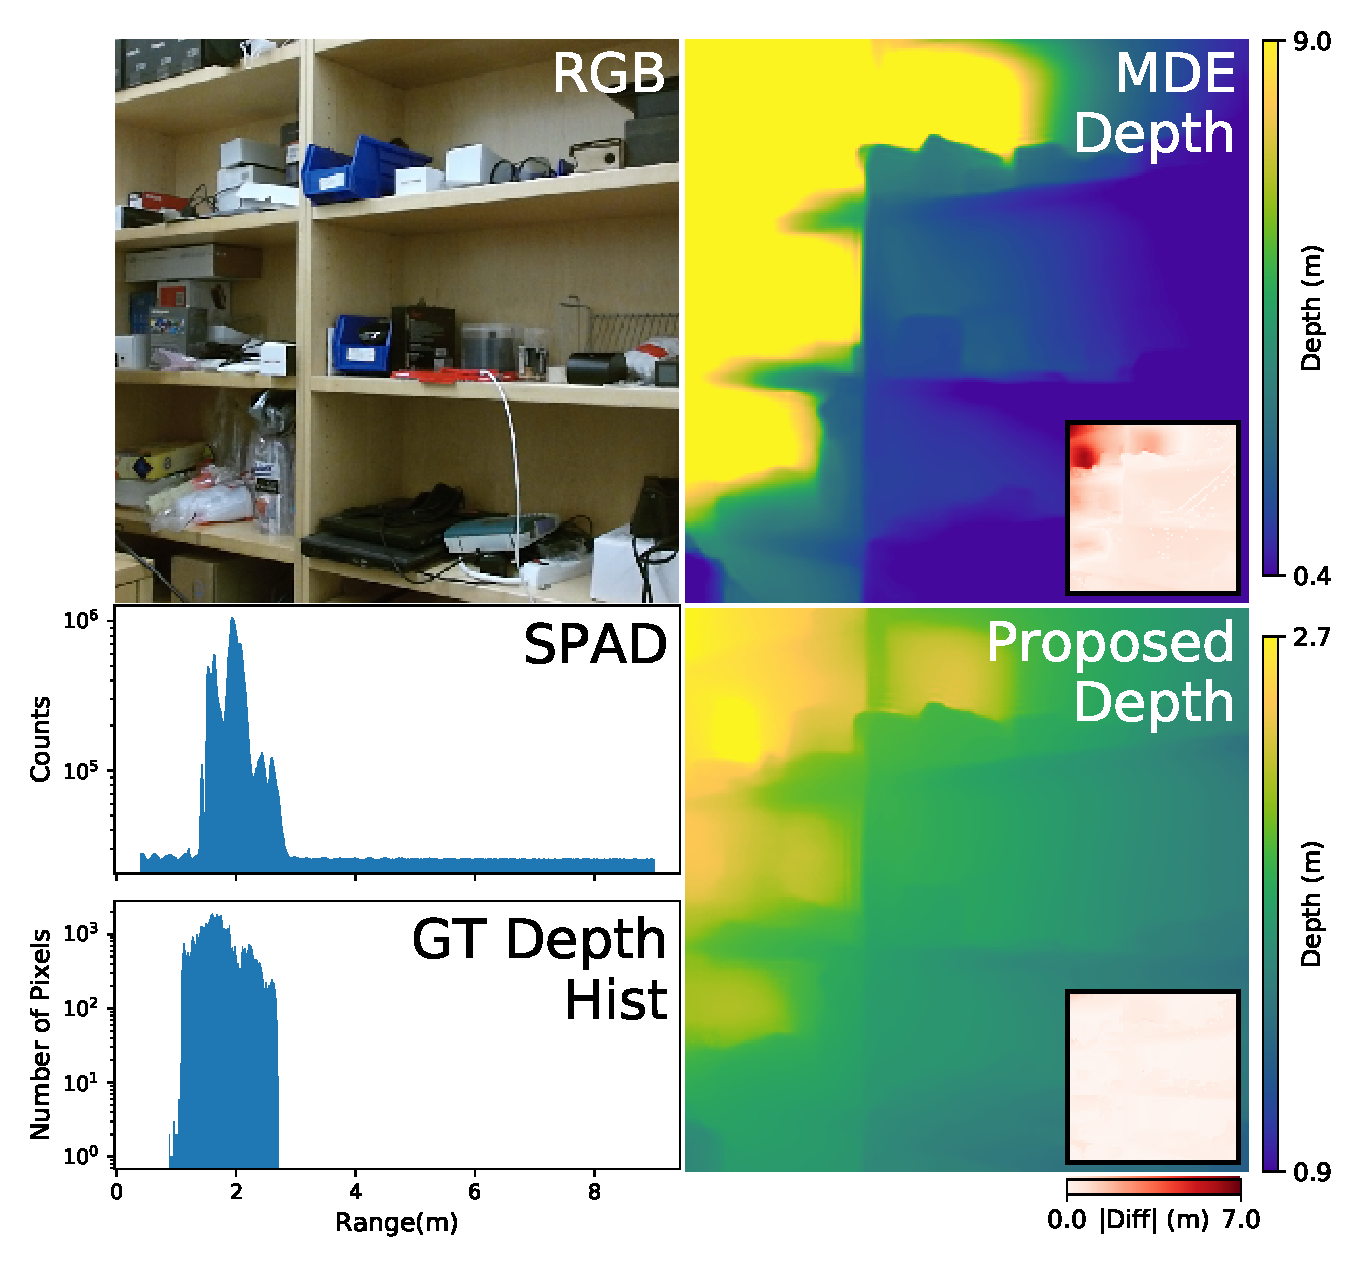
\includegraphics[width=\linewidth]{sections/figures/captured/midas/8_30_small_lab_scene/teaser.eps}
  \caption{Our method uses the SPAD's histogram to rescale the initial depth
    estimate from the CNN to align with the ground truth depth.}
  \label{fig:teaser}
\end{figure}
Our method is not without limitations. It still requires a laser and
single-pixel LiDAR detector, and as such, is sensitive to ambient photons. Being 
a variant of histogram matching, our method is unable to transpose the
values of pixels (i.e. if pixel $a$ is farther
than pixel $b$ in the input, it will be farther than pixel $b$ in the output).
In other words, our method is not able to resolve ordinal depth errors
(errors where an object is wrongly placed closer or farther
relative to another object). Finally, our method is non-differentiable, and is
therefore unsuitable for end-to-end optimization of multi-part networks.

\begin{itemize}
	\item We introduce the idea of augmenting an RGB camera with a global depth 
    histogram to address scale ambiguity error in monocular depth estimators.	
  \item We analyze our approach on indoor scenes using the NYU Depth v2 dataset.
    We demonstrate that our approach is able to resolve scale ambiguity while
    being fast and easy to implement.
	\item We build a hardware prototype and evaluate the efficacy of our
    approach on real-world data, assessing both the the quality and the ability of our method
    to help generalization of monocular depth estimators across scene types. 
\end{itemize}


